\chapter{Revisão de literatura[Fundamentação teórica]}
\thispagestyle{empty}
Em geral, neste capítulo devem ser apresentadas as bases teóricas da sua pesquisa. O capítulo pode ser denominado “Revisão da literatura” (ou “Revisão bibliográfica”) ou “Fundamentação teórica” (ou “Referencial teórico”) consoante seu conteúdo. O termo “Referencial teórico” também pode ser empregado para denominar este capítulo.

“Fundamentação teórica” ou “Referencial teórico”: traz os conceitos básicos e clássicos de física, tecnológicos etc., necessários à compreensão da dissertação.

“Revisão de literatura” ou “Revisão bibliográfica”: é uma retrospectiva do estado da arte sobre o tema da pesquisa, com o objetivo de situar o leitor sobre a situação atual do tema da pesquisa, bem como as lacunas que ainda demanda desenvolvimento. No caso de “Revisão da Literatura” uma detalhada revisão sistemática da literatura deve ser apresentada. Não deve ser feita uma revisão superficial não sistemática, com seleção discricionária e não justificada dos documentos a serem revisados. Deve ser apresentada a estratégia de busca utilizada na revisão sistemática, compreendendo uma seção deste capítulo.

\section{Estratégia de busca}
Caso o capítulo apresente uma revisão da literatura, a estratégia de busca empregada deve ser detalhada. Devem ser apresentados, no mínimo, os seguintes itens:
\begin{itemize}
    \item Termos de busca (simples e compostos)
    \item Critérios de inclusão e exclusão dos documentos
    \item Bases de busca
    \item Recorte temporal (justificado)
    \item Recorte de conteúdo (justificado)
    \item Recorte de língua dos documentos (justificado)
\end{itemize}

\section{Conceitos}
Todo o texto deve ser escrito atendendo a versão mais atual das normas da ABNT. Este guia é apenas orientativo, sendo que os documentos formais de normas de escrita são as versões atualizadas das normas da ABNT.

\section{Breve histórico}
É possível fazer uma revisão da história do tema ou dos principais conceitos que serão utilizados na monografia. Observe que apenas deve ser apresentado o que for relevante para o seu trabalho. É um erro comum o discente incluir vários conceitos fundamentais desnecessários para a compreensão do seu texto, o que o torna enfadonho e pouco atrativo para o leitor.

\section{Linguagem}
Utilize sempre a norma culta da língua portuguesa. Não use gírias, expressões de baixo calão e, principalmente, utilize ortografia correta. Se houver dúvidas sobre a correta escrita de alguma palavra, procure um dicionário da língua portuguesa reconhecido pela Academia Brasileira de Letras (ABL) ou, preferencialmente, o Vocabulário Ortográfico da Língua Portuguesa (VOLP), disponível no site da ABL (ACADEMIA BRASILEIRA DE LETRAS, 2009).

\subsection{Ortografia}
Naturalmente, a ortografia correta é exigência absoluta. Evite anglicismos ou estrangeirismos a menos que sejam absolutamente necessários. Evite usar palavras em língua estrangeira, a menos que tenham sido incorporados ao VOLP. Caso seja absolutamente necessário utilizar palavras em língua estrangeira, estas devem ser grafadas em itálico, seguido do significado entre parênteses.

%Exemplo de Figura

\begin{figure}[H]% H manda colocar exatamente nessa posição no texto (relativa aos parágrafos anterior e %posterior)
	\centering
 	  \caption{Capa da 5ª edição do Vocabulário Ortográfico da Língua Portuguesa}
		\includegraphics{imagens/capavolp.png}
	\label{fig:capavolp}
  \source{disponível em \url{http://www.academia.org.br/nossa-lingua/vocabulario-ortografico}.}
\end{figure}

Segundo a figura \ref{fig:capavolp}.
\subsubsection{Níveis de indentação}
Evite muitos níveis de indentação. Esse é o quarto nível (modelo Título 4). Embora possa haver outros níveis de indentação, 4 níveis é o máximo recomendado.
\subsection{Gramática e estilo}
Empregue sempre a gramática correta no seu texto. Estilo é uma forma individual de escrita. No gênero literário de escrita técnica, o estilo pode variar entre os autores, mas algum rigor deve ser seguido. Nos parágrafos seguintes serão apresentadas algumas dicas que, se seguidas, não serão criticados pela banca e farão seu texto ser mais atrativo para o leitor.

A seguir são apresentados alguns erros típicos de gramática que não devem ocorrer e algumas expressões ou termos que podem ser escritos por questões de estilo.

\begin{enumerate}[label=\alph*)]

{\bfseries \item  Uso da abreviação “etc.”}

O termo “etc.” é a abreviação da expressão em latim “et cetera”, que significa “e outras coisas”. Como trata-se de uma abreviação, deve terminar com um ponto mesmo que esteja no meio da frase, seguindo-se por letra minúscula na palavra subsequente. Se terminar uma frase, basta o ponto de final de período. Como etc. já traz consigo o “e”, não deve ser escrito “e etc.”, nem tampouco deve ser precedido por vírgula. O uso de vírgula antes do etc. pode ser aceito na gramática moderna, mas a linguagem formal tradicional não a permite. Evite usar vírgula antes do etc. Nunca utilize reticências (“...”) após o etc.

{\bfseries \item  Separar sujeito do predicado em uma oração}

O correto uso de vírgulas num texto técnico não é difícil, mas requer a atenção para algumas regras básicas. Um dos erros mais comuns é separar o sujeito do predicado por vírgulas, o que é um erro. Por exemplo:
“As pesquisas realizadas, indicaram que o resultado foi positivo.”
O sujeito desta frase é “as pesquisas realizadas” e o predicado é “indicaram que o resultado foi positivo”. Assim sendo, não pode ser utilizada vírgula para os separar.

{\bfseries \item  Uso do advérbio “mesmo” como pronome}

Esse é um erro fatal que emporcalha o texto. Infelizmente, uma legislação municipal no Rio de Janeiro (e em alguns outros munícipios) propagou um erro de gramática, nos obrigando a ler: “Antes de entrar no elevador, verifique se o mesmo está parado neste andar”. Nesse caso, o termo “mesmo” traz o sentido de um pronome, que se trata de uma classe gramatical da qual o termo “mesmo” não faz parte. O correto seria escrever “Antes de entrar no elevador, verifique se ele está parado neste andar”.

Dica: sempre que for usar o termo “mesmo” ou “mesma”, verifique se pode ser substituído por “ele”, “ela” ou por outro pronome. Se a frase fizer sentido, então não use “mesmo” mas sim o pronome apropriado.
\item {\bfseries Iniciar frase com “E”}

A conjunção aditiva “e” não deve ser utilizado para iniciar. Conjunções são termos que ligam duas ou mais palavras ou orações das mesmas classes gramaticais. Assim sendo, não é gramaticalmente correto iniciar uma frase com conjunção aditiva.

{\bfseries \item  Uso de “e/ou”}

Esse é um tema um tanto controverso. A norma culta da língua portuguesa prescinde do “e/ou” uma vez que o “ou” é não excludente. Isto é, “ou” é uma disjunção não exclusiva, portanto é equivalente ao “e/ou”. Na norma culta, a disjunção exclusiva é dada pelo “ou ... ou”. Por exemplo, para deixar a entender que um laboratório é exclusivamente de calibração ou exclusivamente de ensaio, a norma culta define que seria escrito assim: “... laboratório ou de ensaio ou de calibração”, ou alguma redação semelhante.

Entretanto, vale mencionar que hoje em dia se aceita o “e/ou” em linguagem cotidiana, portanto se trata de estilo usar ou não. Como sugestão, empregue o “e/ou” apenas em casos que a ausência do “e/” venha a trazer confusão no entendimento do texto. Repetindo: o “ou” na língua portuguesa tem o sentido de não exclusividade, portanto já contempla o sentido do “e/”.

{\bfseries \item  Diferença entre ilustração e tabela}

Tabelas são elementos da estrutura de um texto técnico nas quais as principais informações transmitidas são números. Por outro lado, ilustrações podem ser desenhos, esquemas, fluxogramas, fotografias, gráficos, mapas, organogramas, plantas, quadros, retratos etc. Todos estes elementos podem ser genericamente denominados ilustrações, ou especificamente para cada tipo de ilustração. Cada tipo de elemento deve ser enumerado independentemente por ordem de aparecimento no texto. Embora não sejam elementos obrigatórios, geralmente são inseridas listas de tabelas e de ilustrações. A seguir serão apresentados exemplos de tabela, quadro e figura.




%Exemplo de Tabela
\begin{table}[!ht]
		\centering
		\Caption{Quantidade  de dias dos meses do primeiro semestre do ano.}		
		\IBGEtab{}{
		
		    %\resizebox{15cm}{!}{%
		    \begin{adjustbox}{width=0.7\textwidth,center}
			\begin{tabular}{ccccccc}
		    	\toprule
				JAN & FEV & MAR & ABR & MAI & JUN & JUL \\
				\midrule 
				31 & 28 (ou 29) & 31 & 30 & 31 & 30 & 31\\
				\bottomrule
			\end{tabular}
			\end{adjustbox}
		}{
		}
		\source{elaboração própria}
		\label{tab:exemplo-1}
\end{table}


\begin{table}[h]
\centering
\caption{Cotação do dólar turismo na primeira semana de abril de 2020.}
\label{tab:my-table}
\begin{adjustbox}{width=0.4\textwidth,center}
\begin{tabular}{@{}ccc@{}}
\toprule
          & \multicolumn{2}{c}{Cotação em real} \\ \cmidrule(l){2-3} 
Data      & Compra           & Venda            \\
01ABR2020 & 5,2399           & 5,2404           \\
02ABR2020 & 5,2645           & 5,2651           \\
03ABR2020 & 5,2991           & 5,2997           \\
04ABR2020 & --               & --               \\
05ABR2020 & --               & --               \\
06ABR2020 & 5,2465           & 5,2471           \\
07ABR2020 & 5,2211           & 5,2217           \\ \bottomrule
\end{tabular}
\end{adjustbox}
\source{\url{https://www4.bcb.gov.br} [acessado em 23ABR2020].}
\end{table}

    \begin{quadro}[h!]
        \caption{Nomes, símbolos e grandezas das unidades do Sistema Interamericano de Metrologia.}
        % coloque aqui o seu quadro
        \centering
		\includegraphics{imagens/Quadro grandezas.png}
	    \label{qd:grandezas}
	    \source{BIPM.}
    \end{quadro}
    
    %Exemplo de Figura
    
\begin{figure}[htbp]
    \caption{Exemplo de Figura.}
	\centering
		\includegraphics[scale=1]{imagens/barco.png}
	\source{elaboração própria.}
	\label{fig:barco}
\end{figure}

Observe que tanto tabelas quanto ilustrações (todos os tipos) devem ter a seguinte formatação: antes do elemento deve haver um título composto por “tipo” ou “palavra designativa” que pode ser desenho, esquema, fluxograma, fotografia, gráfico, mapa, organograma, planta, quadro, retrato, figura, imagem etc. A palavra designativa deve ser iniciada por letra maiúscula e demais letras minúsculas, seguida por um número de ordem de ocorrência no texto em algarismos arábicos, sucedido por um travessão ladeado por espaços simples (“ – ”) e seguido da descrição do elemento “título”, finalizando com um ponto simples. Após o elemento deve ser apresentada sua fonte mesmo que seja de elaboração própria. A grafia correta é, por exemplo: “Fonte: elaboração própria.”. “Fonte: adaptado de REFERÊNCIA.”; “Fonte: extraído de REFERÊNCIA.”. Observe que “Fonte” inicia-se por letra maiúscula e demais letras são minúsculas, seguindo-se dois pontos (“:”) e o texto a seguir deve ser iniciado por letras minúsculas, salvo nas classes gramaticais que demandar iniciarem-se por letras maiúsculas, como nomes próprios ou siglas, por exemplo. A apresentação da fonte deve ser finalizada por um ponto simples. As normas da ABNT são omissas quanto ao uso de ponto simples para finalizar a descrição do elemento (tabela ou ilustração). Entretanto, este guia faz uso desta formatação. O autor precisa ficar atento quando a fonte citar um site, pois o uso de ponto ao fina do site pode fazê-lo não ser identificado pelo navegador na internet. O tamanho da letra das descrições das tabelas, ilustrações e fontes é menor que a do corpo do texto. Neste guia, o tamanho do corpo do texto é 12 e destes elementos citados é 11 (ambos Times New Roman).

Quanto à formatação, a tabela não deve ter linhas verticais, a menos que sejam relevantes para melhor apresentar as informações. São obrigatórias três linhas horizontais em uma tabela: a que delimita o topo (ou início) da tabela; a que separa o topo do corpo (ou meio) da tabela; e a linha inferior que delimita o final da tabela. Outras linhas horizontais podem ser necessárias para melhor apresentação das informações, mas são dispensáveis. O documento que rege a elaboração de tabelas é o guia gerado pelo IBGE (IBGE, 1993).

{\bfseries \item  Equações e fórmulas}

Todas as unidades devem ser baseadas na edição atual do Sistema Internacional de Unidades (SI). A seguir é apresentado um modelo para equações e fórmulas. As equações devem ser numeradas sequencialmente ao longo do texto e referenciadas no texto.

\begin{equation}
(x+a)^{n}= \sum_{k=0}^{n}\binom{n}{k}x^{k}a^{n-k}
\label{equexemplo}
\end{equation}




Na equação \ref{equexemplo}, \begin{math}x\end{math} é uma variável, \begin{math}a\end{math} é uma constante, \begin{math}n\end{math} é o expoente, \begin{math}k\end{math} é o contador e \begin{math}\sum\end{math} é o símbolo de somatório.

{\bfseries \item  Separação de capítulos}

Cada capítulo da sua monografia deverá se iniciar em uma página distinta da do capítulo anterior. Para isso, não acrescente linhas em branco ao final do capítulo até o título do capítulo subsequente “pular” para a próxima página. Os editores de texto, incluindo o MS Word, dispõem de uma ferramenta denominada “inserir quebra de página”. Fica muito mais elegante e evita perda de formatação caso alguma linha seja retirada ou inserida no capítulo.

{\bfseries \item  Manter linhas de cabeçalho e títulos com o texto que o sucede}

Um erro infelizmente recorrente é a presença de “linhas soltas” no texto. Por exemplo, se for introduzido uma seção no final de uma página, pode ocorrer que o parágrafo subsequente ao título da seção “pule” para a página seguinte. Para evitar isso, use a ferramenta de edição “Manter com o próximo”, ou outra denominação do seu editor de texto. Assim, caso a formatação do texto seja alterada, automaticamente o título da seção irá acompanhar o parágrafo que a sucede.

A mesma observação vale para títulos de tabelas e ilustrações. Use da ferramenta “Manter com o próximo” para que o título fique sempre acima e na mesma página do elemento que o sucede, assim como o próprio elemento com a descrição da fonte, elemento obrigatório e que deve suceder a tabela ou ilustração.

É importante NÃO ACRESCENTAR LINHAS ENTRE AS DESCRIÇÕES DAS TABELAS E ILUSTRAÇÕES E ANTES DA DESCRIÇÃO DA FONTE.

{\bfseries \item  Uso de advérbios}

Os advérbios são fundamentais para uma boa escrita. O grande problema é usá-lo apropriadamente. Recomenda-se uma revisão do tema em alguma gramática de boa qualidade. Essencialmente, deve-se atentar para alguns vícios de linguagem recorrentes. Advérbios são elementos gramaticais que, estando próximos (“ad”) a um verbo, adjetivo alteram seu significado (incluindo um outro advérbio). Um erro comum é usar o advérbio de lugar “onde” com função distinta da sua proposta. Eis um uso inapropriado do adverbio “onde”: “Eu fiz um experimento semana passada onde os resultados foram favoráveis”. Mais correto seria “... semana passada quando os resultados ...” (advérbio de tempo e não de lugar).

Outro erro comum é usar a locução adverbial “através de” com o sentido de “por meio de”. “Através” tem sentido de atravessar, enquanto “por meio de” é uma locução adverbial de modo, podendo ser substituída por “do seguinte modo” ou “de tal maneira”.

{\bfseries \item  Siglas}

O correto é escrever o nome por extenso e a respectiva sigla em seguida, e não o inverso. Por exemplo: Agência Nacional de Aviação Civil (ANAC); Instituto Nacional de Metrologia, Qualidade e Tecnologia (Inmetro).
É possível usar a sigla em inglês e fazer a tradução na descrição. Por exemplo: Comissão Internacional de Eletrotécnica (IEC, do inglês International Eletrotechnical Commission). A partir desta definição, pode ser utilizada a sigla IEC normalmente.

{\bfseries \item  Plural de siglas}

Gramaticalmente, não está errado escrever siglas no plural, mas é uma questão de estilo. Muitos leitores preferem a forma clássica de representar siglas apenas na sua forma original, isto é, no singular. Por exemplo, “Unidade Organizacional” tem como sigla “UO”. Ao se referir a mais de uma UO, o autor pode optar por escrever UOs ou manter a sigla original UO. O sentido da oração se dará pelo artigo que precederá a sigla ou pela flexão do verbo, conforme seja a construção da oração. Veja os exemplos a seguir:

“A UO tem 50 servidores.”

“A UO terá seu orçamento anual majorado em 10\%.”

“As UO têm 50 servidores cada.”

“As UO terão seus orçamentos anuais majorados em 10\%.”

Não há dúvidas que os dois primeiros exemplos dizem respeito a apenas uma UO, enquanto os outros dois exemplos se referem a mais de uma UO. Portanto não é necessário acrescentar a letra “s” após a sigla para transmitir ao leitor a informação que são mais de uma UO.

Observação importante: é absolutamente errado usar ’s (apóstrofe seguido da letra “s”) para representar plural de sigla. Por exemplo, está errado escrever “UO’s”.

Ainda em relação ao uso de siglas, estas devem vir por extenso no ponto do texto onde aparecem pela primeira vez. Por exemplo: Coordenação Geral de Acreditação (Cgcre).

{\bfseries \item  Plural de símbolos}

Símbolos não têm plural! A observação é importante, inclusive, para símbolos das unidades do SI. Não existe plural de A ou N, que são os símbolos das unidades ampere (grandeza corrente elétrica) e newton (grandeza força). Entretanto, à unidade escrita por extenso deve ser acrescentada a letra “s” para representar seu plural: amperes e newtons.

{\bfseries \item  Use linguagem formal e não coloquial}

Expressões coloquiais como, por exemplo “tipo assim”, “levantar as informações” etc. não devem ser empregadas. O texto fica pobre e não irá satisfazer o leitor. Essas expressões são aceitas em textos literários, naturalmente, mas não em textos técnicos e científicos.

{\bfseries \item  Vícios de linguagem}

Na linguagem vulgar ou coloquial, o uso de determinadas construções gramaticais ou de estilo são admitidas. Entretanto, em textos técnicos isso não é permitido. A seguir são apresentados alguns exemplos mais comuns. O autor da monografia deve estar atento para não cometer esses ou outros vícios de linguagem.
\begin{itemize}
    \item Usar “através” ao invés de “por meio de”. Exemplo: “As medições foram feitas através de um multímetro”. O correto seria “As medições foram feitas por meio de um multímetro” ou “... com uso de ...”.
    \item 	A expressão “período de tempo” está incorreta. “Período” é uma grandeza equivalente a “tempo”.
\end{itemize}

{\bfseries \item  Referências bibliográficas}

A norma ABNT NBR 6023 apresenta como devem ser elaboradas as referências bibliográficas, elemento pós-textual obrigatório. A citação no corpo do texto deve seguir o previsto na ABNT NBR 10520. Apesar de haver algumas formas de se citarem as referências (sistema de chamadas), a preferencial para monografias é “AUTOR-DATA” (veja cláusula 6.1 da ABNT NBR 10520). A manutenção das referências em um texto longo é muito mais simples quando a lista das referências está em ordem alfabética e não em ordem de aparição no texto. Estude as normas ABNT NBR 10520 e ABNT NBR 6023 para citar apropriadamente as referências na monografia.

Vale observar que o capítulo REFERÊNCIAS BIBLIOGRÁFICAS tem o mesmo nível hierárquico das seções principais (INTRODUÇÃO, REVISÃO BIBLIOGRÁFICA, METODOLOGIA, RESULTADOS, DISCUSSÃO e CONCLUSÃO), mas não é numerado.

A lista de referências diz muito sobre a qualidade do artigo. Deve-se evitar citações bibliográficas em português a menos que sejam estritamente necessárias. Normas, por exemplo, é sempre mais aconselhável citar a versão internacional, se houver, ou similar. Nunca cite teses ou dissertações. Uma boa tese ou dissertação terá gerado artigo em períódico. Procure artigos dos autores daquela tese ou dissertação sobre o assunto. Evite ao máximo citar artigos de congressos. Revistas técnicas e científicas são a melhor fonte de bibliografia técnica e acadêmica, preferencialmente com DOI. Livros, cite pouco e apenas os clássicos.

{\bfseries \item  Coesão textual}

Ao escrever, lembre-se que seu texto como um todo deve fazer sentido para o leitor. O autor, num texto dissertativo (ou mesmo numa tese), busca convencer o leitor acerca de um determinado assunto. Por isso, evite ao máximo inserir mudanças repentinas de assunto ao longo do seu texto. Caso seja preciso mudar de assunto numa mesma seção do seu trabalho, faça-o de maneira elegante, como por exemplo por meio da inserção de parágrafos de ligação.

A transição na exposição de ideias ao longo do seu texto deve ser feita com coerência e lógica, de forma que o texto seja coeso (ou contínuo).Na língua portuguesa há elementos que conferem coesão a um texto. Tratam-se de expressões que estabelecem a transição de ideias entre frases e parágrafos, como pronomes, advérbios e conjunções.

    \begin{quadro}[h!]
        \caption{Exemplos de elementos de coesão textual.}
        % coloque aqui o seu quadro
        \centering
		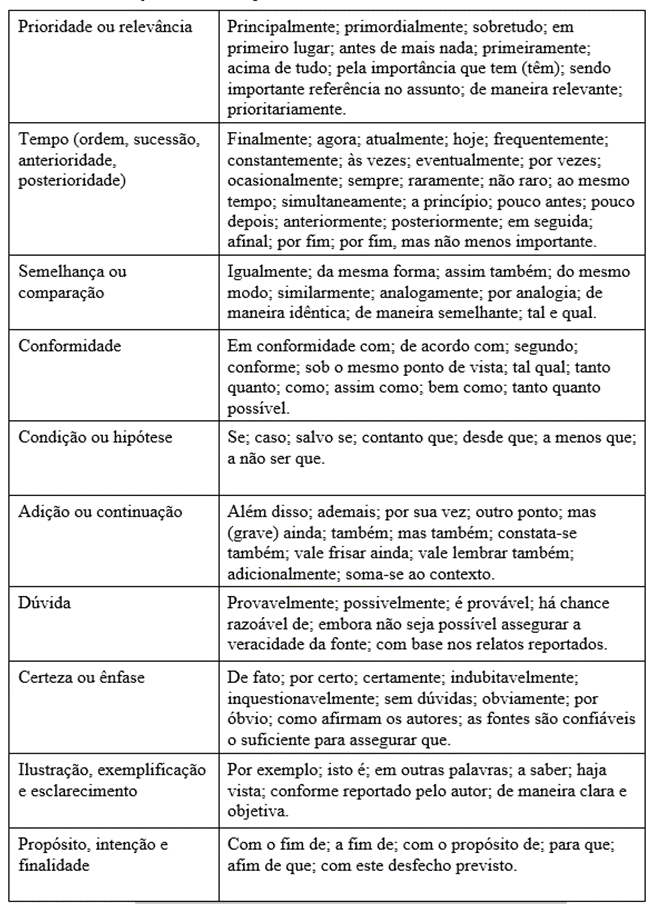
\includegraphics[scale=0.8]{imagens/quadro2.png}
	    \label{qd:grandezas}
	    \source{adaptado de \citeonline{Borges}, com acréscimos de autoria própria.}
    \end{quadro}

\end{enumerate}